\chapter{C\`{a}lculs B\`{a}sics}\label{sec:calc_bas}

Es tracten en aquest cap\'{\i}tol c\`{a}lculs b\`{a}sics, que poden servir en la
resoluci\'{o} de diversos problemes electrot\`{e}cnics.

\section{\texorpdfstring{Transformaci\'{o} estrella $\boldsymbol{\leftrightarrow}$ triangle d'imped\`{a}ncies}
    {Transformaci\'{o} estrella-triangle d'imped\`{a}ncies}}\label{secc:d_y} \index{transformaci\'{o}
estrella $\leftrightarrow$ triangle}

En un sistema trif\`{a}sic, pot interessar transformar tres imped\`{a}ncies connectades en
estrella, en tres imped\`{a}ncies equivalents connectades en triangle
$(\text{Y}\rightarrow\Delta)$, o a l'inrev\'{e}s, transformar tres imped\`{a}ncies connectades en
triangle, en tres imped\`{a}ncies equivalents connectades en estrella
$(\Delta\rightarrow\text{Y})$. Atenent a la Figura \vref{pic:Y_D}, tenim les seg\"{u}ents
transformacions:
\begin{equation}\label{eq:Y_D}
   \text{Y}\rightarrow\Delta\;\left\{
   \begin{array}{lll}
      \cmplx{Z}_{\alphaup\betaup} &= &\displaystyle \cmplx{Z}_{\alphaup} + \cmplx{Z}_{\betaup} + \frac{\cmplx{Z}_{\alphaup}\,\cmplx{Z}_{\betaup}}{\cmplx{Z}_{\gammaup}}  \\[2.5ex]
      \cmplx{Z}_{\betaup\gammaup} &= &\displaystyle \cmplx{Z}_{\betaup} + \cmplx{Z}_{\gammaup} + \frac{\cmplx{Z}_{\betaup}\,\cmplx{Z}_{\gammaup}}{\cmplx{Z}_{\alphaup}}  \\[2.5ex]
      \cmplx{Z}_{\gammaup\alphaup} &= &\displaystyle \cmplx{Z}_{\gammaup} + \cmplx{Z}_{\alphaup} + \frac{\cmplx{Z}_{\gammaup}\, \cmplx{Z}_{\alphaup}}{\cmplx{Z}_{\betaup}}
   \end{array}
   \right.
   \qquad\qquad
   \Delta\rightarrow\text{Y}\;\left\{
   \begin{array}{lll}
      \cmplx{Z}_{\alphaup} &= &\dfrac{\cmplx{Z}_{\alphaup\betaup}\, \cmplx{Z}_{\gammaup\alphaup}}{  \cmplx{Z}_{\alphaup\betaup} + \cmplx{Z}_{\betaup\gammaup}+ \cmplx{Z}_{\gammaup\alphaup}}  \\[2.5ex]
      \cmplx{Z}_{\betaup} &= &\dfrac{\cmplx{Z}_{\betaup\gammaup}\, \cmplx{Z}_{\alphaup\betaup}}{  \cmplx{Z}_{\alphaup\betaup} + \cmplx{Z}_{\betaup\gammaup}+ \cmplx{Z}_{\gammaup\alphaup}}  \\[2.5ex]
      \cmplx{Z}_{\gammaup} &= &\dfrac{\cmplx{Z}_{\gammaup\alphaup}\, \cmplx{Z}_{\betaup\gammaup}}{  \cmplx{Z}_{\alphaup\betaup} + \cmplx{Z}_{\betaup\gammaup}+ \cmplx{Z}_{\gammaup\alphaup}}
   \end{array}
   \right.
\end{equation}

\begin{figure}[htb]
    \centering
    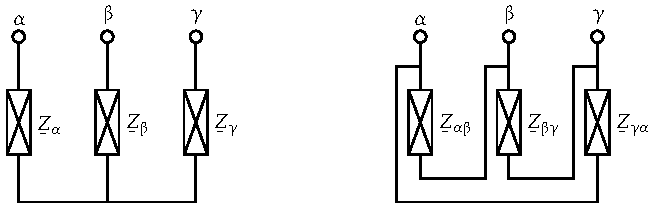
\includegraphics{Imatges/Cap-CalcBas-YD.pdf}
\caption{Transformaci\'{o} estrella $\leftrightarrow$ triangle
d'imped\`{a}ncies} \label{pic:Y_D}
\end{figure}

\begin{exemple}
Es vol transformar tres imped\`{a}ncies connectades en triangle, de
valors $ \cmplx{Z}_{\alphaup\betaup}=10\unit{\ohm}$,
$\cmplx{Z}_{\betaup\gammaup}=-\ju10\unit{\ohm}$ i
$\cmplx{Z}_{\gammaup\alphaup}=-\ju10\unit{\ohm}$, en tres imped\`{a}ncies
equivalents connectades en estrella.

A partir de les equacions \eqref{eq:Y_D}  tenim:
\begin{align*}
   \cmplx{Z}_{\alphaup} & = \frac{10\unit{\ohm}\cdot(-\ju10\unit{\ohm})}{10\unit{\ohm} - \ju10\unit{\ohm} - \ju10\unit{\ohm}} = 4 - \ju 2\unit{\ohm} \\[1.5ex]
   \cmplx{Z}_{\betaup} & = \frac{-\ju10\unit{\ohm}\cdot10\unit{\ohm}}{10\unit{\ohm} - \ju10\unit{\ohm} - \ju10\unit{\ohm}} = 4 - \ju 2\unit{\ohm} \\[1.5ex]
\cmplx{Z}_{\gammaup} &=
\frac{-\ju10\unit{\ohm}\cdot(-\ju10\unit{\ohm})}{10\unit{\ohm} -
\ju10\unit{\ohm} - \ju10\unit{\ohm}} = -2 - \ju 4\unit{\ohm}
\end{align*}

\'{E}s possible, com en aquest cas pel que fa a $\cmplx{Z}_{\gammaup}$,
obtenir un valor amb una part real negativa (resist\`{e}ncia negativa);
no obstant, encara que no existeixi f\'{\i}sicament aquesta resist\`{e}ncia,
el seu valor \'{e}s matem\`{a}ticament correcte i es pot utilitzar en
c\`{a}lculs subseg\"{u}ents.
\end{exemple}


\section{Resoluci\'{o} de circuits coneixent la pot\`{e}ncia absorbida per la
c\`{a}rrega}\label{sec:EZS}

Es tracta en aquest apartat la resoluci\'{o} de circuits simples,
formats per una font de tensi\'{o} en s\`{e}rie amb una imped\`{a}ncia, la qual
alimenta a una c\`{a}rrega; aquesta c\`{a}rrega no est\`{a} definida per la seva
imped\`{a}ncia o admit\`{a}ncia, sin\'{o} per la pot\`{e}ncia que absorbeix\footnote{Aquest \'{e}s un cas particular
del problema del flux de c\`{a}rregues en
sistemes el\`{e}ctrics de pot\`{e}ncia, el qual es tracta en el cap\'{\i}tol \ref{chap:flux_carregues}}.

En la Figura \vref{pic:EZS} es representen els circuits que es volen
resoldre, tant per a corrent continu com per a corrent altern. $E$,
$R$ i $P$ (o $\cmplx{E}$, $\cmplx{Z}$ i $\cmplx{S}$) s\'{o}n els valors
coneguts, i $U$ i $I$ (o $\cmplx{U}$ i $\cmplx{I}$) s\'{o}n els valors
que es vol trobar.
\begin{figure}[htb]
\vspace{3mm} \centering
   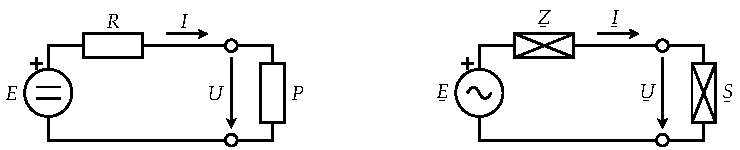
\includegraphics{Imatges/Cap-CalcBas-EZS.pdf}
\caption{Resoluci\'{o} de circuits coneixent la pot\`{e}ncia absorbida per la c\`{a}rrega} \label{pic:EZS}
\end{figure}

\subsection{Circuits de corrent continu}

A partir del circuit de l'esquerra de la Figura \vref{pic:EZS} tenim les dues equacions seg\"{u}ents:
\begin{align}
   E &= R I + U \label{eq:ERP_1} \\
   P &= U I     \label{eq:ERP_2}
\end{align}

Multiplicant l'equaci\'{o} \eqref{eq:ERP_1} per $U$ i substituint l'equaci\'{o} \eqref{eq:ERP_2} en aquest resultat, tenim:
\begin{equation}
   E U = R I U + U^2 = R P + U^2 \quad \rightarrow \quad U^2 - E U + R P = 0 \label{eq:ERP_3}
\end{equation}

A partir de les equacions descrites anteriorment, el circuit es resol seguint els seg\"{u}ents passos:
\begin{dingautolist}{'312}
   \item Obtenim $U$, resolent l'equaci\'{o} de 2n grau \eqref{eq:ERP_3}.
   \item Dels dos valors reals que obtenim, ens quedem amb el m\'{e}s elevat. Si en lloc de dos valors reals, obtingu\'{e}ssim
   un parell de valors conjugats complexos, aix\`{o} ens indicaria que el circuit no t\'{e} una soluci\'{o} f\'{\i}sicament possible, i per tant no seria resoluble.
   \item Finalment, calculem $I$ substituint el valor trobat de $U$ en l'equaci\'{o} \eqref{eq:ERP_2}.
\end{dingautolist}

Un cop trobats $U$ i $I$, podem calcular el valor de la resist\`{e}ncia
$R\ped{P}$ de la c\`{a}rrega, la qual absorbeix la pot\`{e}ncia $P$, a
partir de l'equaci\'{o} \eqref{eq:ERP_2} i de la relaci\'{o} $U =R\ped{P}
I$:
\begin{equation}
   R\ped{P} = \frac{U}{I} = \frac{P}{I^2} = \frac{U^2}{P}
\end{equation}

\subsection{Circuits de corrent altern}

A partir del circuit de la dreta de la Figura \vref{pic:EZS} tenim les dues equacions seg\"{u}ents:
\begin{align}
   \cmplx{E} &= \cmplx{Z} \, \cmplx{I} + \cmplx{U} \label{eq:EZS_1} \\
   \cmplx{S} &= \cmplx{U} \, \cmplx{I}^*           \label{eq:EZS_2}
\end{align}

Conjugant l'equaci\'{o} \eqref{eq:EZS_1}, multiplicant-la per $\cmplx{U}$ i substituint l'equaci\'{o} \eqref{eq:EZS_2} en aquest resultat, tenim:
\begin{equation}
   \cmplx{E}^* \, \cmplx{U} = \cmplx{Z}^* \cmplx{I}^* \, \cmplx{U} + \cmplx{U}^* \, \cmplx{U} =
   \cmplx{Z}^* \, \cmplx{S} + |\cmplx{U}|^2 \quad \rightarrow \quad
   |\cmplx{U}|^2 - \cmplx{E}^* \, \cmplx{U} + \cmplx{Z}^* \, \cmplx{S} = 0
   \label{eq:EZS_3}
\end{equation}

Fem a continuaci\'{o} una rotaci\'{o} dels vectors $\cmplx{E}$ i
$\cmplx{U}$, de valor $\eu^{-\ju\delta}$, on $\delta$ \'{e}s l'argument
del vector $\cmplx{E}$; d'aquesta manera, el nou vector $E'$ tan
sols tindr\`{a} part real, i el nou vector $\cmplx{U}'$ estar\`{a} rotat
respecte del vector $\cmplx{U}$.
\begin{align}
   \delta &= \arg(\cmplx{E}) \label{eq:EZS_9} \\
   E' &= \cmplx{E} \, \eu^{-\ju\delta} = |\cmplx{E}|  \label{eq:EZS_4} \\
   \cmplx{U}' &= \cmplx{U} \, \eu^{-\ju\delta}   \label{eq:EZS_5}
\end{align}

Expressem a continuaci\'{o} l'equaci\'{o} \eqref{eq:EZS_3} utilitzant
aquests dos nous vectors:
\begin{equation}
   |\cmplx{U}'|^2 - E' \, \cmplx{U}' + \cmplx{Z}^* \, \cmplx{S} = 0 \label{eq:EZS_6}
\end{equation}

Finalment, separem l'equaci\'{o} \eqref{eq:EZS_6} en dues, una per a la part real i una altra per a la part imagin\`{a}ria. Cal tenir en compte que $|\cmplx{U}'|^2$ nom\'{e}s t\'{e} part real, de valor $\Re^2(\cmplx{U}') + \Im^2(\cmplx{U}')$.
\begin{align}
   \Re^2(\cmplx{U}') + \Im^2(\cmplx{U}') - E' \, \Re(\cmplx{U}') + \Re(\cmplx{Z}^* \, \cmplx{S}) &= 0 \label{eq:EZS_7} \\
   - E' \, \Im(\cmplx{U}') + \Im(\cmplx{Z}^* \, \cmplx{S}) &= 0 \label{eq:EZS_8}
\end{align}

A partir de les equacions descrites anteriorment, el circuit es resol seguint els seg\"{u}ents passos:
\begin{dingautolist}{'312}
   \item Calculem $E'$ a partir de l'equaci\'{o} \eqref{eq:EZS_4}
   \item Obtenim $\Im(\cmplx{U}')$, resolent l'equaci\'{o} \eqref{eq:EZS_8}.
   \item Substitu\"{\i}m el valor obtingut per a $\Im(\cmplx{U}')$ en l'equaci\'{o} \eqref{eq:EZS_7}, i obtenim $\Re(\cmplx{U}')$ resolent aquesta equaci\'{o} de 2n grau.
   \item Dels dos valors reals que obtenim, ens quedem amb el m\'{e}s elevat. Si en lloc de dos valors reals, obtingu\'{e}ssim un parell de valors conjugats complexos, aix\`{o} ens indicaria que el circuit no t\'{e} una soluci\'{o} f\'{\i}sicament possible, i per tant no seria resoluble.
   \item A partir del valor  obtingut per a $\cmplx{U}'$ en el passos anteriors, i del valor de $\delta$ obtingut a partir de l'equaci\'{o} \eqref{eq:EZS_9}, calculem el valor buscat de $\cmplx{U}$, utilitzant l'equaci\'{o} \eqref{eq:EZS_5}
   \item Finalment, calculem $\cmplx{I}$ substituint el valor trobat de $\cmplx{U}$ en l'equaci\'{o} \eqref{eq:EZS_2}
\end{dingautolist}

Un cop trobats $\cmplx{U}$ i $\cmplx{I}$, podem calcular el valor de
la imped\`{a}ncia  $\cmplx{Z}\ped{S}$ de la c\`{a}rrega, la qual absorbeix
la pot\`{e}ncia $\cmplx{S}$, a partir de l'equaci\'{o} \eqref{eq:EZS_2} i de
la relaci\'{o} $\cmplx{U} = \cmplx{Z}\ped{S} \cmplx{I}$:
\begin{equation}
   \cmplx{Z}\ped{S} = \frac{\cmplx{U}}{\cmplx{I}} =
   \frac{\cmplx{S}}{|\cmplx{I}|^2} =
   \frac{|\cmplx{U}|^2}{\cmplx{S}^*} \label{eq:EZS 10}
\end{equation}

\begin{exemple}
Resoldre el circuit de la dreta de la Figura \vref{pic:EZS}, donats el seg\"{u}ents valors en p.u.:
\[
   \cmplx{E} = 0{,}4 + \ju 0{,}3 \qquad \cmplx{Z} = \ju 0{,}1 \qquad
   \cmplx{S} = 0{,}6 + \ju 0{,}45
\]

Calculem primer $\delta$ i $E'$, segons les equacions \eqref{eq:EZS_9} i \eqref{eq:EZS_4},
i $\cmplx{Z}^* \cmplx{S}$:
\begin{align*}
   \delta &= \arg(0{,}4 + \ju 0{,}3) = 0{,}6435\unit{rad} \\
   E' &= |0{,}4 + \ju 0{,}3| = 0{,5} \\
   \cmplx{Z}^* \cmplx{S} &= - \ju 0{,}1 \cdot (0{,}6 + \ju 0{,}45) = 0{,}045 - \ju 0{,}06
\end{align*}

Calculem a continuaci\'{o} $\Im(\cmplx{U}')$, segons l'equaci\'{o} \eqref{eq:EZS_8}:
\[
   \Im(\cmplx{U}') = \frac{\Im(\cmplx{Z}^* \cmplx{S})}{E'} = \frac{-0{,}06}{0{,}5} = -0{,}12
\]

Formem a continuaci\'{o} el polinomi de 2n grau en $\Re(\cmplx{U}')$ i el resolem, segons l'equaci\'{o} \eqref{eq:EZS_7}:
\begin{align*}
   \Re^2(\cmplx{U}') + (-0{,}12)^2 - 0{,}5 \cdot \Re(\cmplx{U}') + 0{,}045 &= 0 \\
   \Re^2(\cmplx{U}') - 0{,}5 \cdot \Re(\cmplx{U}') + 0{,}0594 &= 0  \;\rightarrow\; \Re(\cmplx{U}') =
   \left\{ \begin{matrix}
     0{,}1943 \\
     \boxed{0{,}3057}
   \end{matrix}
   \right.
\end{align*}

Prenent el valor m\'{e}s elevat de $\Re(\cmplx{U}')$ calculem finalment $\cmplx{U}$, segons l'equaci\'{o} \eqref{eq:EZS_5}:
\[
   \cmplx{U} = \cmplx{U}' \, \eu^{\ju \delta} = (0{,}3057 - \ju 0{,}12) \cdot \eu^{\ju 0{,}6435} =
   0{,}3165 + \ju 0{,}0874
\]

Obtenim ara $\cmplx{I}$, segons l'equaci\'{o} \eqref{eq:EZS_2}:
\[
   \cmplx{I} = \frac{\cmplx{S}^*}{\cmplx{U}^*} = \frac{0{,}6-\ju 0{,}45}{0{,}3165 - \ju 0{,}0874}
   = 2{,}1262 - \ju 0{,}8347
\]

Per acabar, calculem $\cmplx{Z}\ped{S}$, segons l'equaci\'{o}
\eqref{eq:EZS 10}:
\[
    \cmplx{Z}\ped{S} = \frac{\cmplx{U}}{\cmplx{I}} = \frac{0{,}3165 + \ju 0{,}0874}
    {2{,}1262 - \ju 0{,}8347} = 0{,}1150 + \ju 0{,}0863
\]

\end{exemple}



\section{Corrent de curt circuit en el  secundari d'un transformador}
\index{corrent de curt circuit!en el  secundari d'un transformador}

 Es tracta en aquest apartat, el c\`{a}lcul del corrent de curt
circuit trif\`{a}sic en el secundari d'un transformador, que t\'{e} el
primari connectat  a una xarxa de pot\`{e}ncia.

A partir de la Figura \vref{pic:cc_sec_trafo}, es tracta de trobar
el valor del corrent de curt circuit trif\`{a}sic $I\ped{F}$ en el punt
F, essent la resta de par\`{a}metres valors coneguts.

\begin{figure}[htb]
\vspace{3mm} \centering
    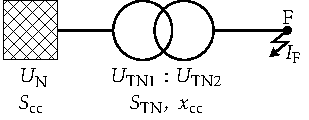
\includegraphics{Imatges/Cap-CalcBas-Icc-Trafo.pdf}
\caption{Corrent de curt circuit en el  secundari d'un
transformador} \label{pic:cc_sec_trafo}
\end{figure}

$U\ped{N}$, $U\ped{TN1}$ i $U\ped{TN2}$ estan donats en volt,
$S\ped{cc}$ i $S\ped{TN}$ en volt ampere, i $x\ped{cc}$ en p.u.
respecte dels valors nominals del transformador.


Per tal de simplificar el problema, suposarem que tant la imped\`{a}ncia
de curt circuit del transformador, com la imped\`{a}ncia equivalent de
la xarxa de pot\`{e}ncia s\'{o}n totalment inductives; d'aquesta manera,
podrem treballar amb les diverses variables implicades, com si
fossin nombres reals. Suposarem a m\'{e}s, que no hi ha circulaci\'{o} de
corrent abans del curt circuit.

Pel que fa a la xarxa de pot\`{e}ncia, si en lloc de la pot\`{e}ncia de curt
circuit $S\ped{cc}$, el que coneixem \'{e}s el corrent de curt circuit
disponible $I\ped{cc}$, podem obtenir el valor de la pot\`{e}ncia de
curt circuit a partir de l'expressi\'{o}:
\begin{equation}
    S\ped{cc} = \sqrt{3} U\ped{N} I\ped{cc}
\end{equation}
\index{pot\`{e}ncia de curt circuit}

 Si prenem com a valors base els
par\`{a}metres del transformador ($U\ped{TN1}$, $U\ped{TN2}$ i
$S\ped{TN}$), la relaci\'{o} de transformaci\'{o} i la imped\`{a}ncia de curt
circuit del transformador, expressats en p.u., seran 1:1 i
$x\ped{cc}$ respectivament. An\`{a}logament, la tensi\'{o} i la imped\`{a}ncia
equivalents de la xarxa de pot\`{e}ncia, expressats en p.u., seran
$\frac{U\ped{N}}{U\ped{TN1}}$ i $\frac{U\ped{N}^2}{S\ped{cc}}
\frac{S\ped{TN}}{U\ped{TN1}^2}$ respectivament.

Amb aquests valors, el corrent de curt circuit $i\ped{F}$, expressat
en p.u., val:
\begin{equation}
    i\ped{F} = \frac{\dfrac{U\ped{N}}{U\ped{TN1}}}{\dfrac{U\ped{N}^2}{S\ped{cc}}
    \dfrac{S\ped{TN}}{U\ped{TN1}^2} + x\ped{cc}}
\end{equation}

I per tant, aquest corrent $I\ped{F}$, expressat en ampere, val:
\begin{equation}
    I\ped{F} = i\ped{F}\; \frac{S\ped{TN}}{\sqrt{3}U\ped{TN2}} =
    \frac{S\ped{TN} U\ped{N}}{\sqrt{3} U\ped{TN1}U\ped{TN2}
    \left(\dfrac{U\ped{N}^2}{S\ped{cc}}
    \dfrac{S\ped{TN}}{U\ped{TN1}^2} + x\ped{cc}\right)}
\end{equation}

Si la xarxa de pot\`{e}ncia es considera de pot\`{e}ncia infinita, tenim:
\begin{equation}
    I\ped{F} = \frac{S\ped{TN} U\ped{N}}{\sqrt{3} U\ped{TN1}U\ped{TN2}
    x\ped{cc}}\qquad\qquad (\text{amb }S\ped{cc}=\infty)
\end{equation}

Si a m\'{e}s, la tensi\'{o} de la xarxa coincideix amb la tensi\'{o} prim\`{a}ria
del transformador, tenim respectivament:
\begin{align}
    I\ped{F} &= \frac{S\ped{TN}}{\sqrt{3} U\ped{TN2}
    \left(\dfrac{S\ped{TN}}{S\ped{cc}} +
    x\ped{cc}\right)}\qquad\qquad(\text{amb }U\ped{N}=U\ped{TN1})\\[1ex]
    I\ped{F} &= \frac{S\ped{TN}}{\sqrt{3} U\ped{TN2}
    x\ped{cc}}\qquad\qquad(\text{amb }U\ped{N}=U\ped{TN1}\text{ i }
    S\ped{cc}=\infty)
\end{align}

\begin{exemple}
A partir de la Figura \vref{pic:cc_sec_trafo}, amb els valors
$U\ped{N}=6900\unit{V}$, $U\ped{TN1}=6900\unit{V}$,
$U\ped{TN2}=400\unit{V}$, $S\ped{TN}=850\unit{kVA}$ i
$x\ped{cc}=5\unit{\%}$, es tracta de trobar $I\ped{F}$ en el cas
que: a) $S\ped{cc}=200\unit{MVA}$ i b) $S\ped{cc}=\infty$.

El valors demanats s\'{o}n:
\begin{align*}
   &a)\;I\ped{F} = \frac{850\unit{kVA}}{\sqrt{3}\cdot 400\unit{V}\cdot
   \left(\dfrac{850\unit{kVA}}{200\unit{MVA}} +
   0{,}05\right)} = 22{,}6\unit{kA} \\[1ex]
   &b)\;I\ped{F} = \frac{850\unit{kVA}}{\sqrt{3}\cdot 400\unit{V}\cdot
   0{,}05} = 24{,}5\unit{kA}
\end{align*}

\end{exemple}


\section{Escales logar\'{\i}tmiques} \index{escales logar\'{\i}tmiques}

En diferents camps de l'electrot\`{e}cnia, \'{e}s usual trobar-se gr\`{a}fics amb escales
logar\'{\i}tmiques.

Un exemple clar, s\'{o}n els gr\`{a}fics d'actuaci\'{o} dels interruptors magnetot\`{e}rmics o dels
fusibles, on les seves corbes caracter\'{\i}stiques intensitat--temps estan representades en
una escala logar\'{\i}tmica--logar\'{\i}tmica o lineal--logar\'{\i}tmica.

En aquests casos, es presenta freq\"{u}entment la necessitat de determinar amb exactitud un
punt de la corba, que no coincideix amb cap de les l\'{\i}nies divis\`{o}ries del gr\`{a}fic. Atenent a
la Figura \vref{pic:escala log}, es tractaria de determinar el valor $x$ dins de la d\`{e}cada
$10^N$ a $10^{N+1}$.

\begin{figure}[htb]
\vspace{5mm} \centering
    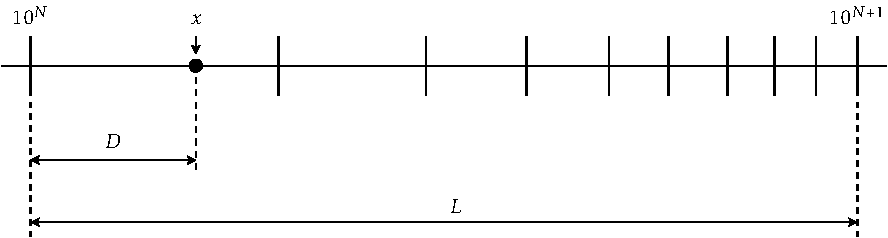
\includegraphics{Imatges/Ape-EscalesLog.pdf}
\caption{Escala logar\'{\i}tmica} \label{pic:escala log}
\end{figure}

Si mesurem amb un regle la dist\`{a}ncia $D$ des de l'inici de la d\`{e}cada fins al punt $x$, i
la longitud total $L$ de la d\`{e}cada, el valor $x$ buscat ve donat per l'expressi\'{o}:
\begin{equation}
    x = 10^{\left(N+\frac{D}{L}\right)}
\end{equation}

Si estem interessats en el problema invers, \'{e}s a dir, en  trobar la dist\`{a}ncia $D$
corresponent a un valor conegut $x$ dins de la d\`{e}cada $10^N$ a $10^{N+1}$, podem emprar
l'expressi\'{o}:
\begin{equation}
    D = L(\log x - N) = L \log\frac{x}{10^N}
\end{equation}

\begin{exemple}
Es tracta de trobar el valor $x$ dins de la d\`{e}cada 100 a 1000, corresponent a una
dist\`{a}ncia $D=11\unit{mm}$; la longitud total de la d\`{e}cada \'{e}s $L=56\unit{mm}$.

En aquest cas tenim $N=2$, i per tant:
\[
    x = 10^{\left(2+\frac{11\unit{mm}}{56\unit{mm}}\right)}= 157{,}19
\]
\end{exemple}

\begin{exemple}
Es tracta de trobar la dist\`{a}ncia $D$ a la qual hem de dibuixar el valor $x=5$, dins de la
d\`{e}cada 1 a 10; la longitud total de la d\`{e}cada \'{e}s $L=56\unit{mm}$.

En aquest cas tenim $N=0$, i per tant:
\[
    D = 56\unit{mm} \cdot (\log 5 - 0)  = 39{,}1\unit{mm}
\]
\end{exemple}

